\subsubsection{Komplettsystem}
\begin{figure}[h!]
	\centering
	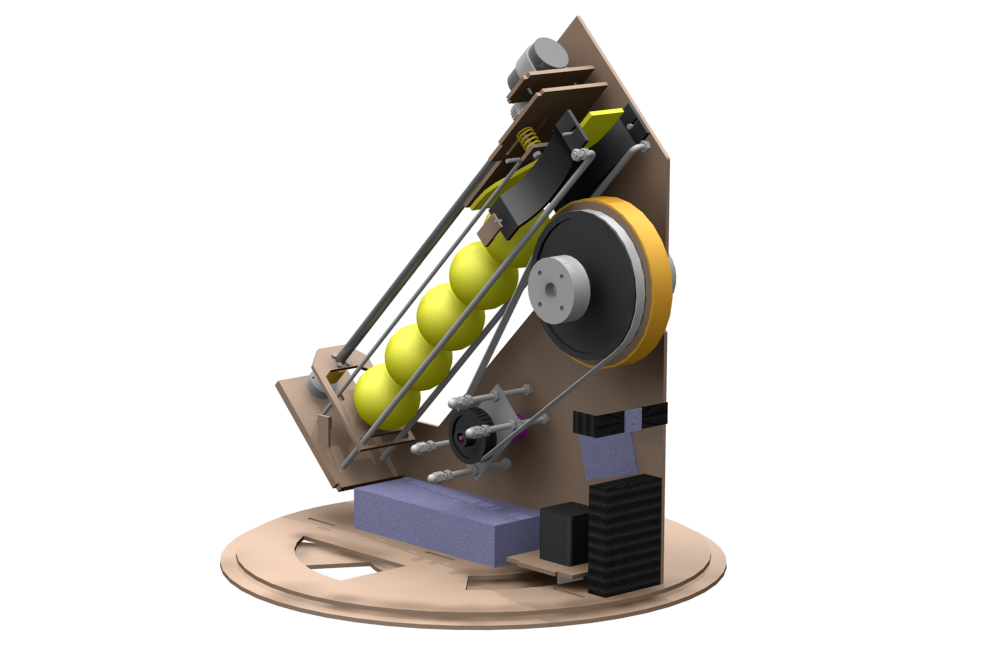
\includegraphics[width=\linewidth]{../../fig/Render_Komplettsystem_5}
	\caption{Komplettsystem}
	\label{fig:Komplettsystem}
\end{figure}
\paragraph{Komponentenbeschrieb\\}
Das System ist in die Teilsysteme "`Ausrichtung Drehturm"', "`Ballnachschub"', "`Drehturm"', "`Anpressvorrichtung"' und "`Wurfmechanismus"' unterteilt. Nachfolgend wird auf die einzelnen Komponenten genauer eingegangen. Um die verschiedenen gelaserten Komponenten zu verbinden sind vorwiegend Steckverbindungen eingesetzt. Um dies zu ermöglichen sind den Einzelteilen Aussparungen und Nuten beigefügt. Anbaukomponenten wie Lager oder Halterungen sind mit Schraub-, sowie vereinzelt Klebeverbindungen befestigt. Die zwei Grundplatten sind mit eingepressten Stiften verbunden.

\paragraph{Entwicklungsprozess\\}
Für die Entwicklung der Wurfmaschine wurden diverse Handskizzen erstellt. Nach Auswahl des Konzeptes, visualisierte und entwickelte man alle weiteren Ideen mittels dem CAD-Programm Siemens NX8 bzw. NX9. Durch dieses Vorgehen konnten Änderungen jeweils schnell angebracht werden. Für einige mechanische Komponenten wurden detaillierte technische Zeichnungen erstellt, um sie in der schulinterne mechanischen Werkstätte fertigen zu lassen. Bei der Entwicklung wurde der Stabilität des Aufbaus grosse Beachtung geschenkt. Dadurch hatten wir während der Testphase keinerlei Probleme mit zerstörten Bauteilen oder behelfsmässigen Anpassungen. Das Gewicht fällt dadurch jedoch höher aus. 